\documentclass[11pt,varwidth=500px]{standalone}
\usepackage{amsmath,amssymb,calc,ifthen}
\usepackage{float}
%\usepackage{cancel}
\usepackage[table,usenames,dvipsnames]{xcolor} % for coloured cells in tables
\usepackage{tikz}
% Allows us to click on links and references!
\usepackage{hyperref}
\usepackage{url}
\hypersetup{
colorlinks,
citecolor=black,
filecolor=black,
linkcolor=black,
urlcolor=black
}
% Nice package for plotting graphs
% See excellent guide:
% http://www.tug.org/TUGboat/tb31-1/tb97wright-pgfplots.pdf
\usetikzlibrary{plotmarks,shapes}
\usepackage{amsmath,graphicx}
\usepackage{epstopdf}
\usepackage{caption}
\usepackage{subcaption}
\usepackage{graphicx}
% highlight - useful for TODOs and similar
\usepackage{color}
\newcommand{\hilight}[1]{\colorbox{yellow}{#1}}
\newcommand\ci{\perp\!\!\!\perp} % perpendicular sign
\newcommand*\rfrac[2]{{}^{#1}\!/_{#2}} % diagonal fraction
\newcommand\SLASH{\char`\\}
\usepackage{listings}
% margin size
\usepackage[margin=1.0in]{geometry}
\usepackage{pdfpages}
\usepackage{enumitem} % for nested enumerate numbers 1 1.1 1.1.1

\usepackage{titlesec} % reduce spacing after subsections

\usepackage[percent]{overpic}

% \titlespacing\subsection{0pt}{4pt plus 4pt minus 2pt}{4pt plus 2pt minus 2pt}
\captionsetup{justification=centering}

\begin{document}
\belowdisplayskip=12pt plus 3pt minus 9pt
\belowdisplayshortskip=7pt plus 3pt minus 4pt

\newcommand{\figScale}{0.5}

\begin{figure}[H]
 \centering
 
%  \textbf{\huge{A}}
 \begin{subfigure}{0.47\textwidth}
%  \begin{picture}(7,7)
%     \put(-0,-10){}
%     \end{picture}
%     \begin{overpic}[scale=\figScale,tics=10]{fig1_linReg.png}
%  \put (20,55) {\textbf{\huge{A}}}
% \end{overpic}

    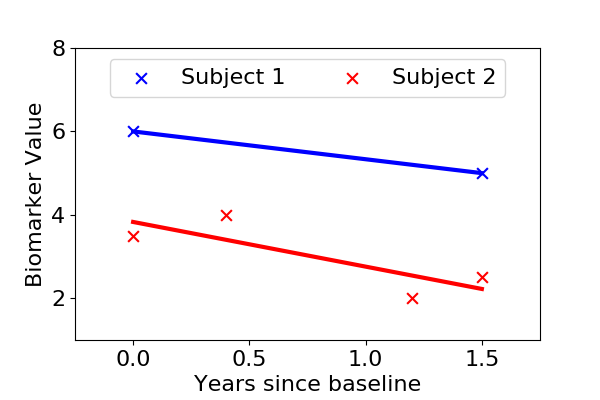
\includegraphics[width=\textwidth]{fig1_linReg.png}
    \begin{picture}(7,7)
    \put(0,150){\textbf{\huge{A}}}
    \end{picture}
 \end{subfigure}
 \begin{subfigure}{0.47\textwidth}
     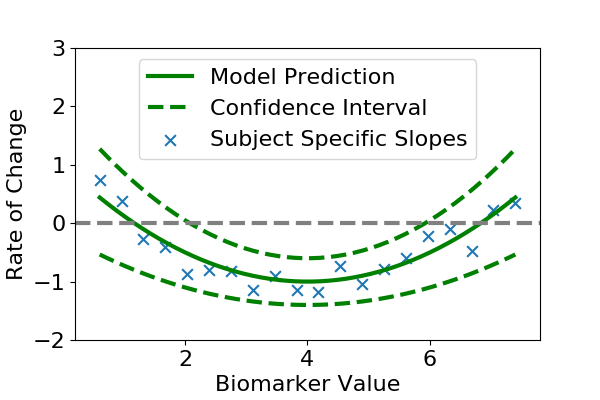
\includegraphics[width=\textwidth]{fig2_GP.png}
     \begin{picture}(7,7)
    \put(0,150){\textbf{\huge{B}}}
    \end{picture}
 \end{subfigure}
 \vspace{1em}
 
  \begin{subfigure}{0.47\textwidth}
    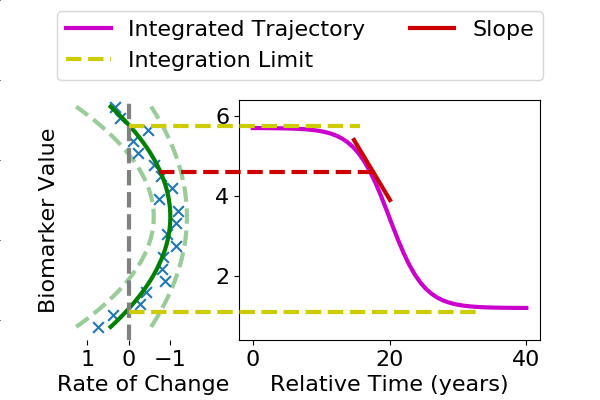
\includegraphics[width=\textwidth]{fig3_recon.png}
\begin{picture}(7,7)
    \put(0,150){\textbf{\huge{C}}}
    \end{picture}
 \end{subfigure}
 \begin{subfigure}{0.47\textwidth}
     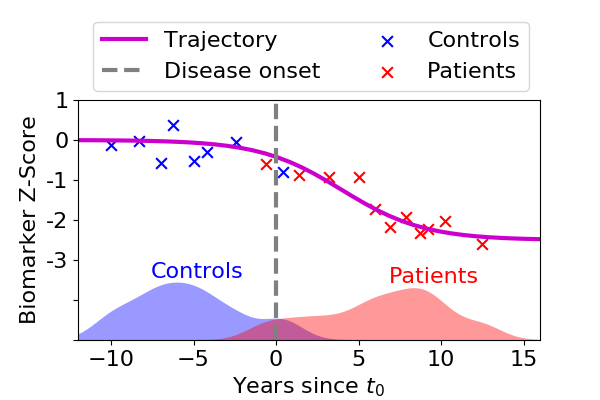
\includegraphics[width=\textwidth]{fig4_align.png}
\begin{picture}(7,7)
    \put(0,150){\textbf{\huge{D}}}
    \end{picture}
 \end{subfigure}
 
% \caption{Diagram of the Differential Equation Model. (a) Measuring biomarker rate of change from line of best fit: The biomarker measurements for each subject were plotted against time since baseline, and a line was fit for each subject independently. The slope of these lines was then used as a measure of the biomarker rate of change (b) Rate of change model: The slopes of each fitted line were plotted against the average biomarker value of each subject (blue crosses). A non-parametric model (Gaussian Process) were then fitted on measurements, which gave a model prediction and also a 95\% confidence interval. For example, if a biomarker value of four corresponds to a rate of change equal to minus one, it means that in a year's time the biomarker value will decrease to three. (c) Trajectory reconstruction: A line integral was performed on the rate of change model from figure (2). The integration limits were defined as the biomarker values where the corresponding change is zero. Starting from the upper integration limit, the trajectory was reconstructed from the rate of change prediction, which represents the slope corresponding to that biomarker value. Before integration, an arbitrary starting time point, $t_0 = 0$, was defined, thus all time is relative to $t_0$. (d) Anchoring process: to give an absolute estimate of time since disease onset, the origin $t_0$ was set so that the trajectory prediction at $t+0$ is equal to the average biomarker value of patients at baseline. Moreover, to make trajectories comparable across biomarkers we convert the biomarker values to Z-scores with respect to controls, which results in a scaling along the Y-axis. The process (a-d) was repeated for each biomarker independently. After fitting every biomarker, the subjects can be staged along the disease timeline, as in Fig. (d), using the trajectories from all biomarkers.
% }
\end{figure}


%'incrSubj'    'incrDistOverlap'    'incrMisData'    'incrBiomk'    'incrStagingUnif'    'incrCtlPrec'



\end{document}





















